\chapter{Appendix A}

\section{Additional Apparatus Pictures} \label{sec:additional_apparatus}

\begin{figure}[htpb]
    \centering
    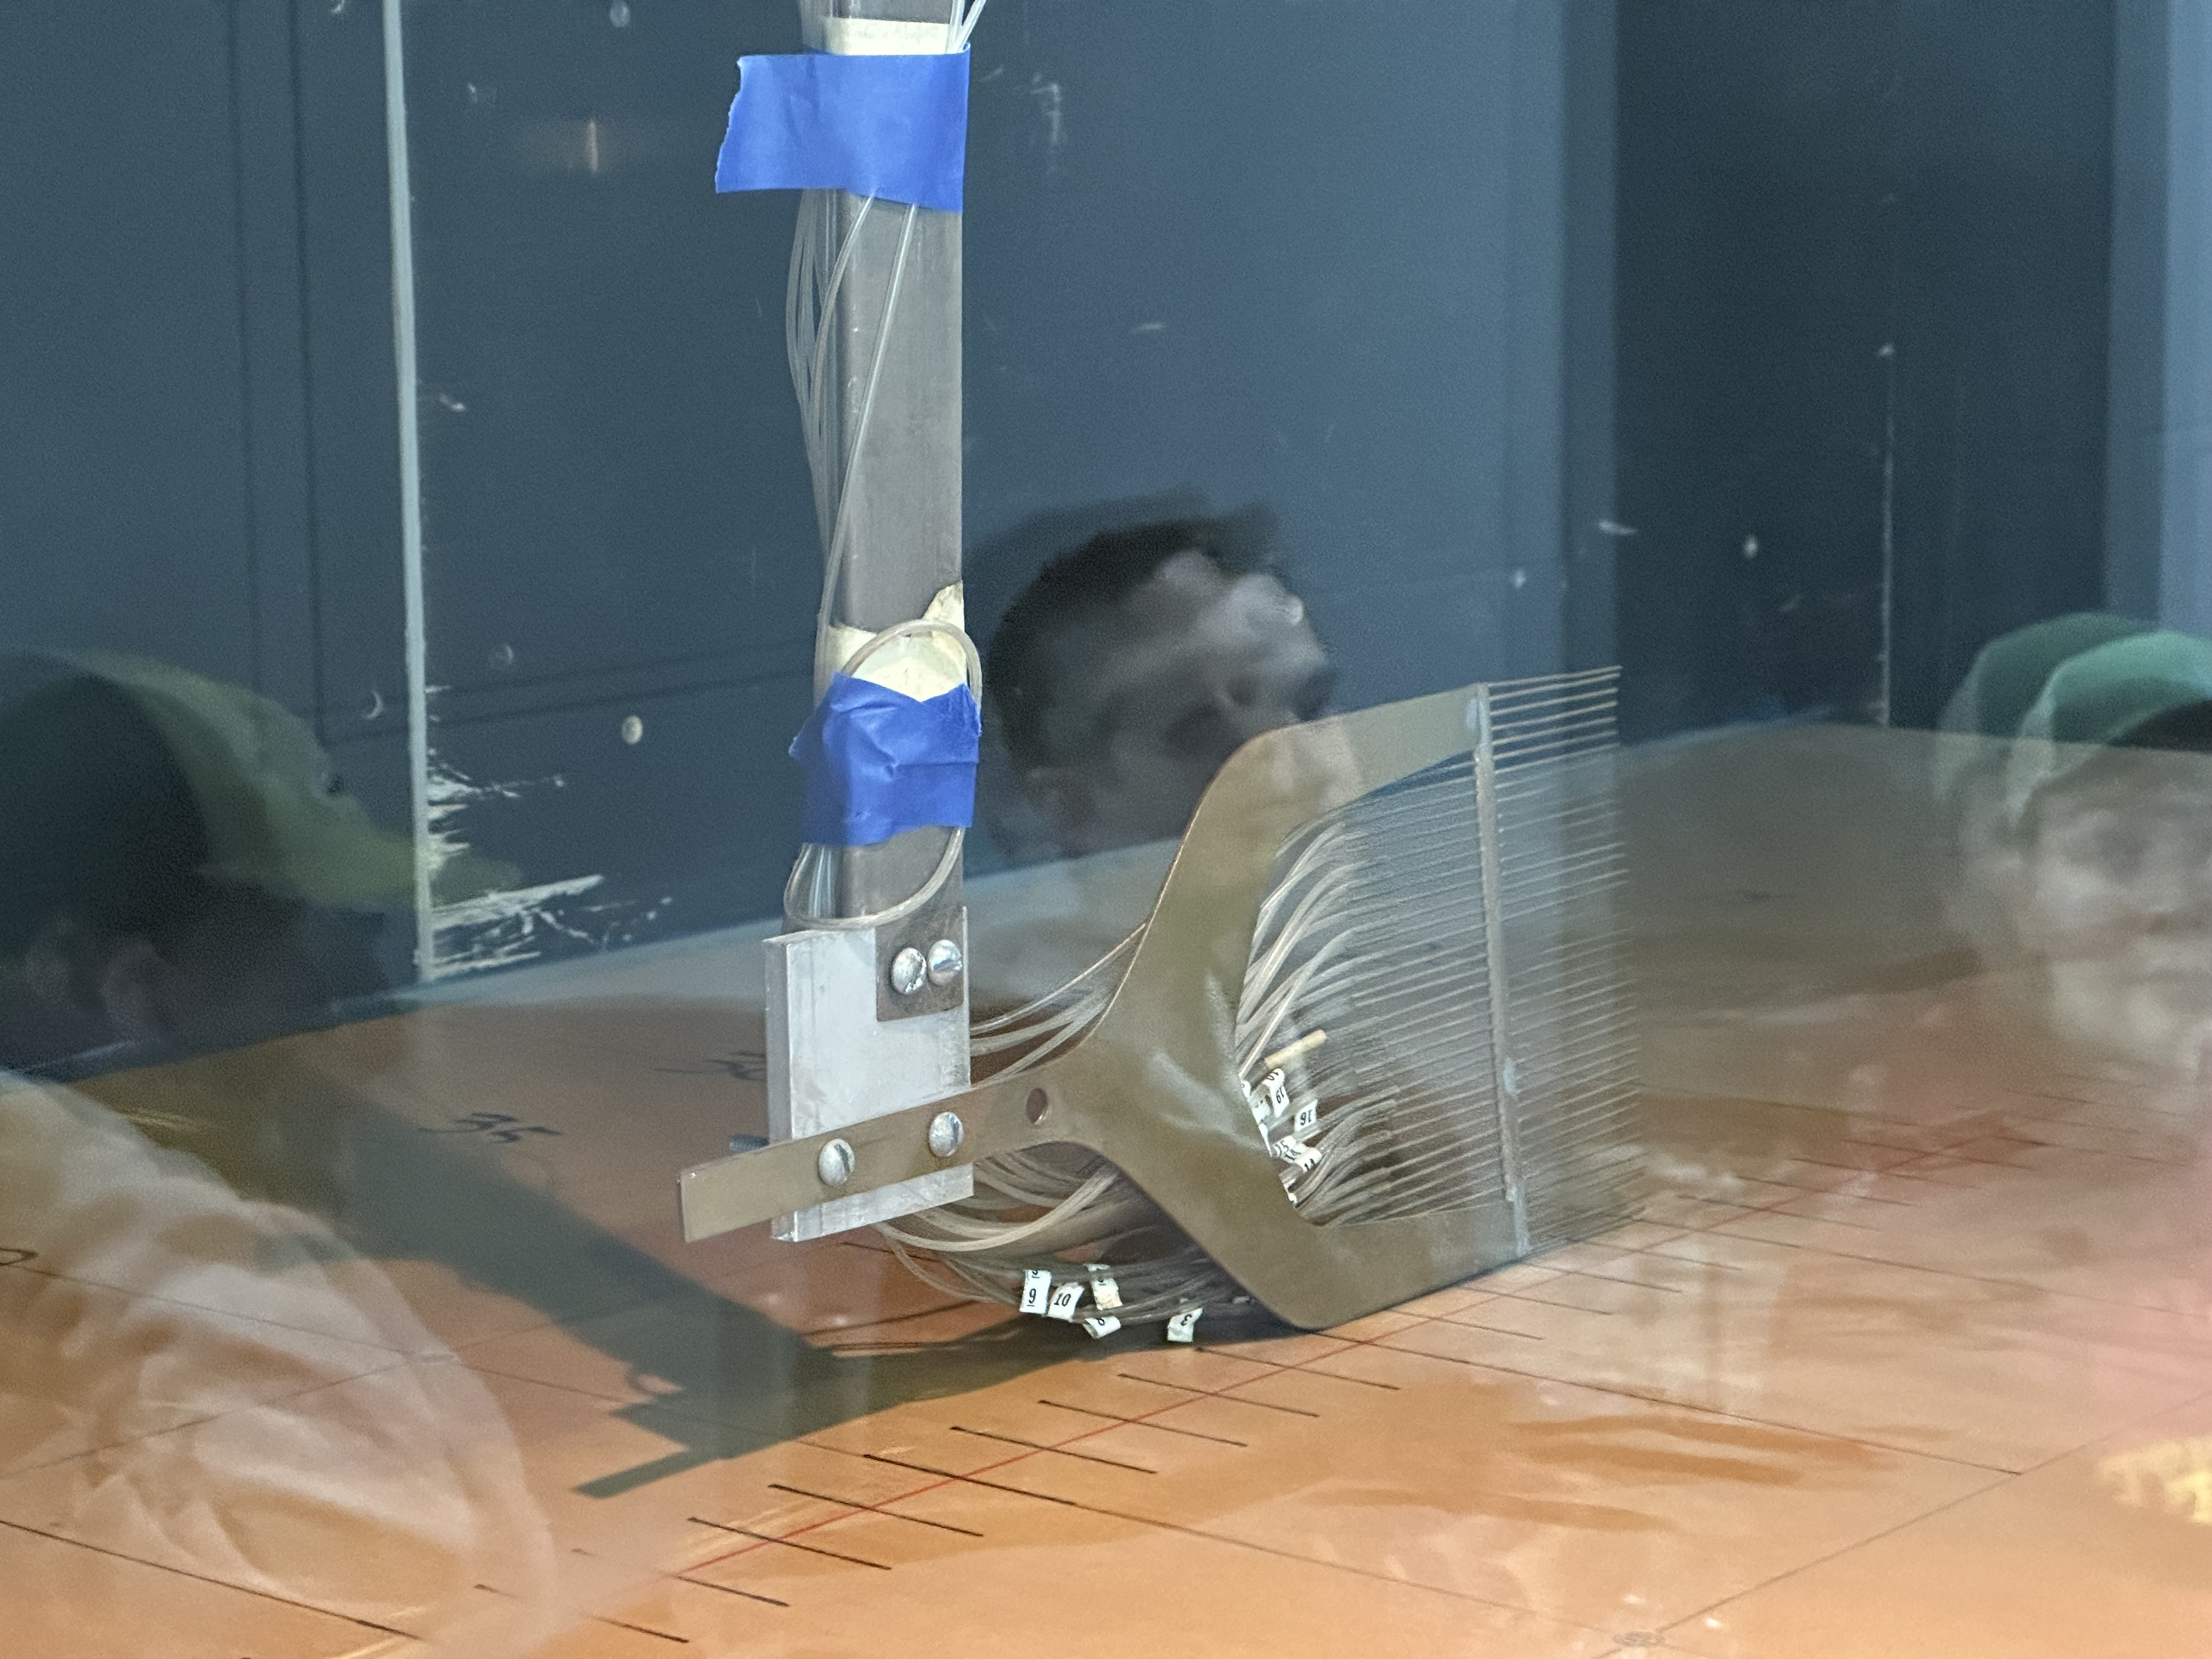
\includegraphics[width=0.75\linewidth]{Figures/IMG_0002.jpeg}
    \caption[Pressure Rake in open circuit wind tunnel]{Pressure rake in open circuit wind tunnel}
    \label{fig: PressureRake}
\end{figure}

\begin{figure}[htpb]
    \centering
    \includegraphics[width=0.75\linewidth]{Figures/IMG_0005.jpeg}
    \caption[Picture of the flat plate in test section]{Picture of the flat plate in test section}
    \label{fig: FlatPlate}
\end{figure}

\begin{figure}[htpb]
    \centering
    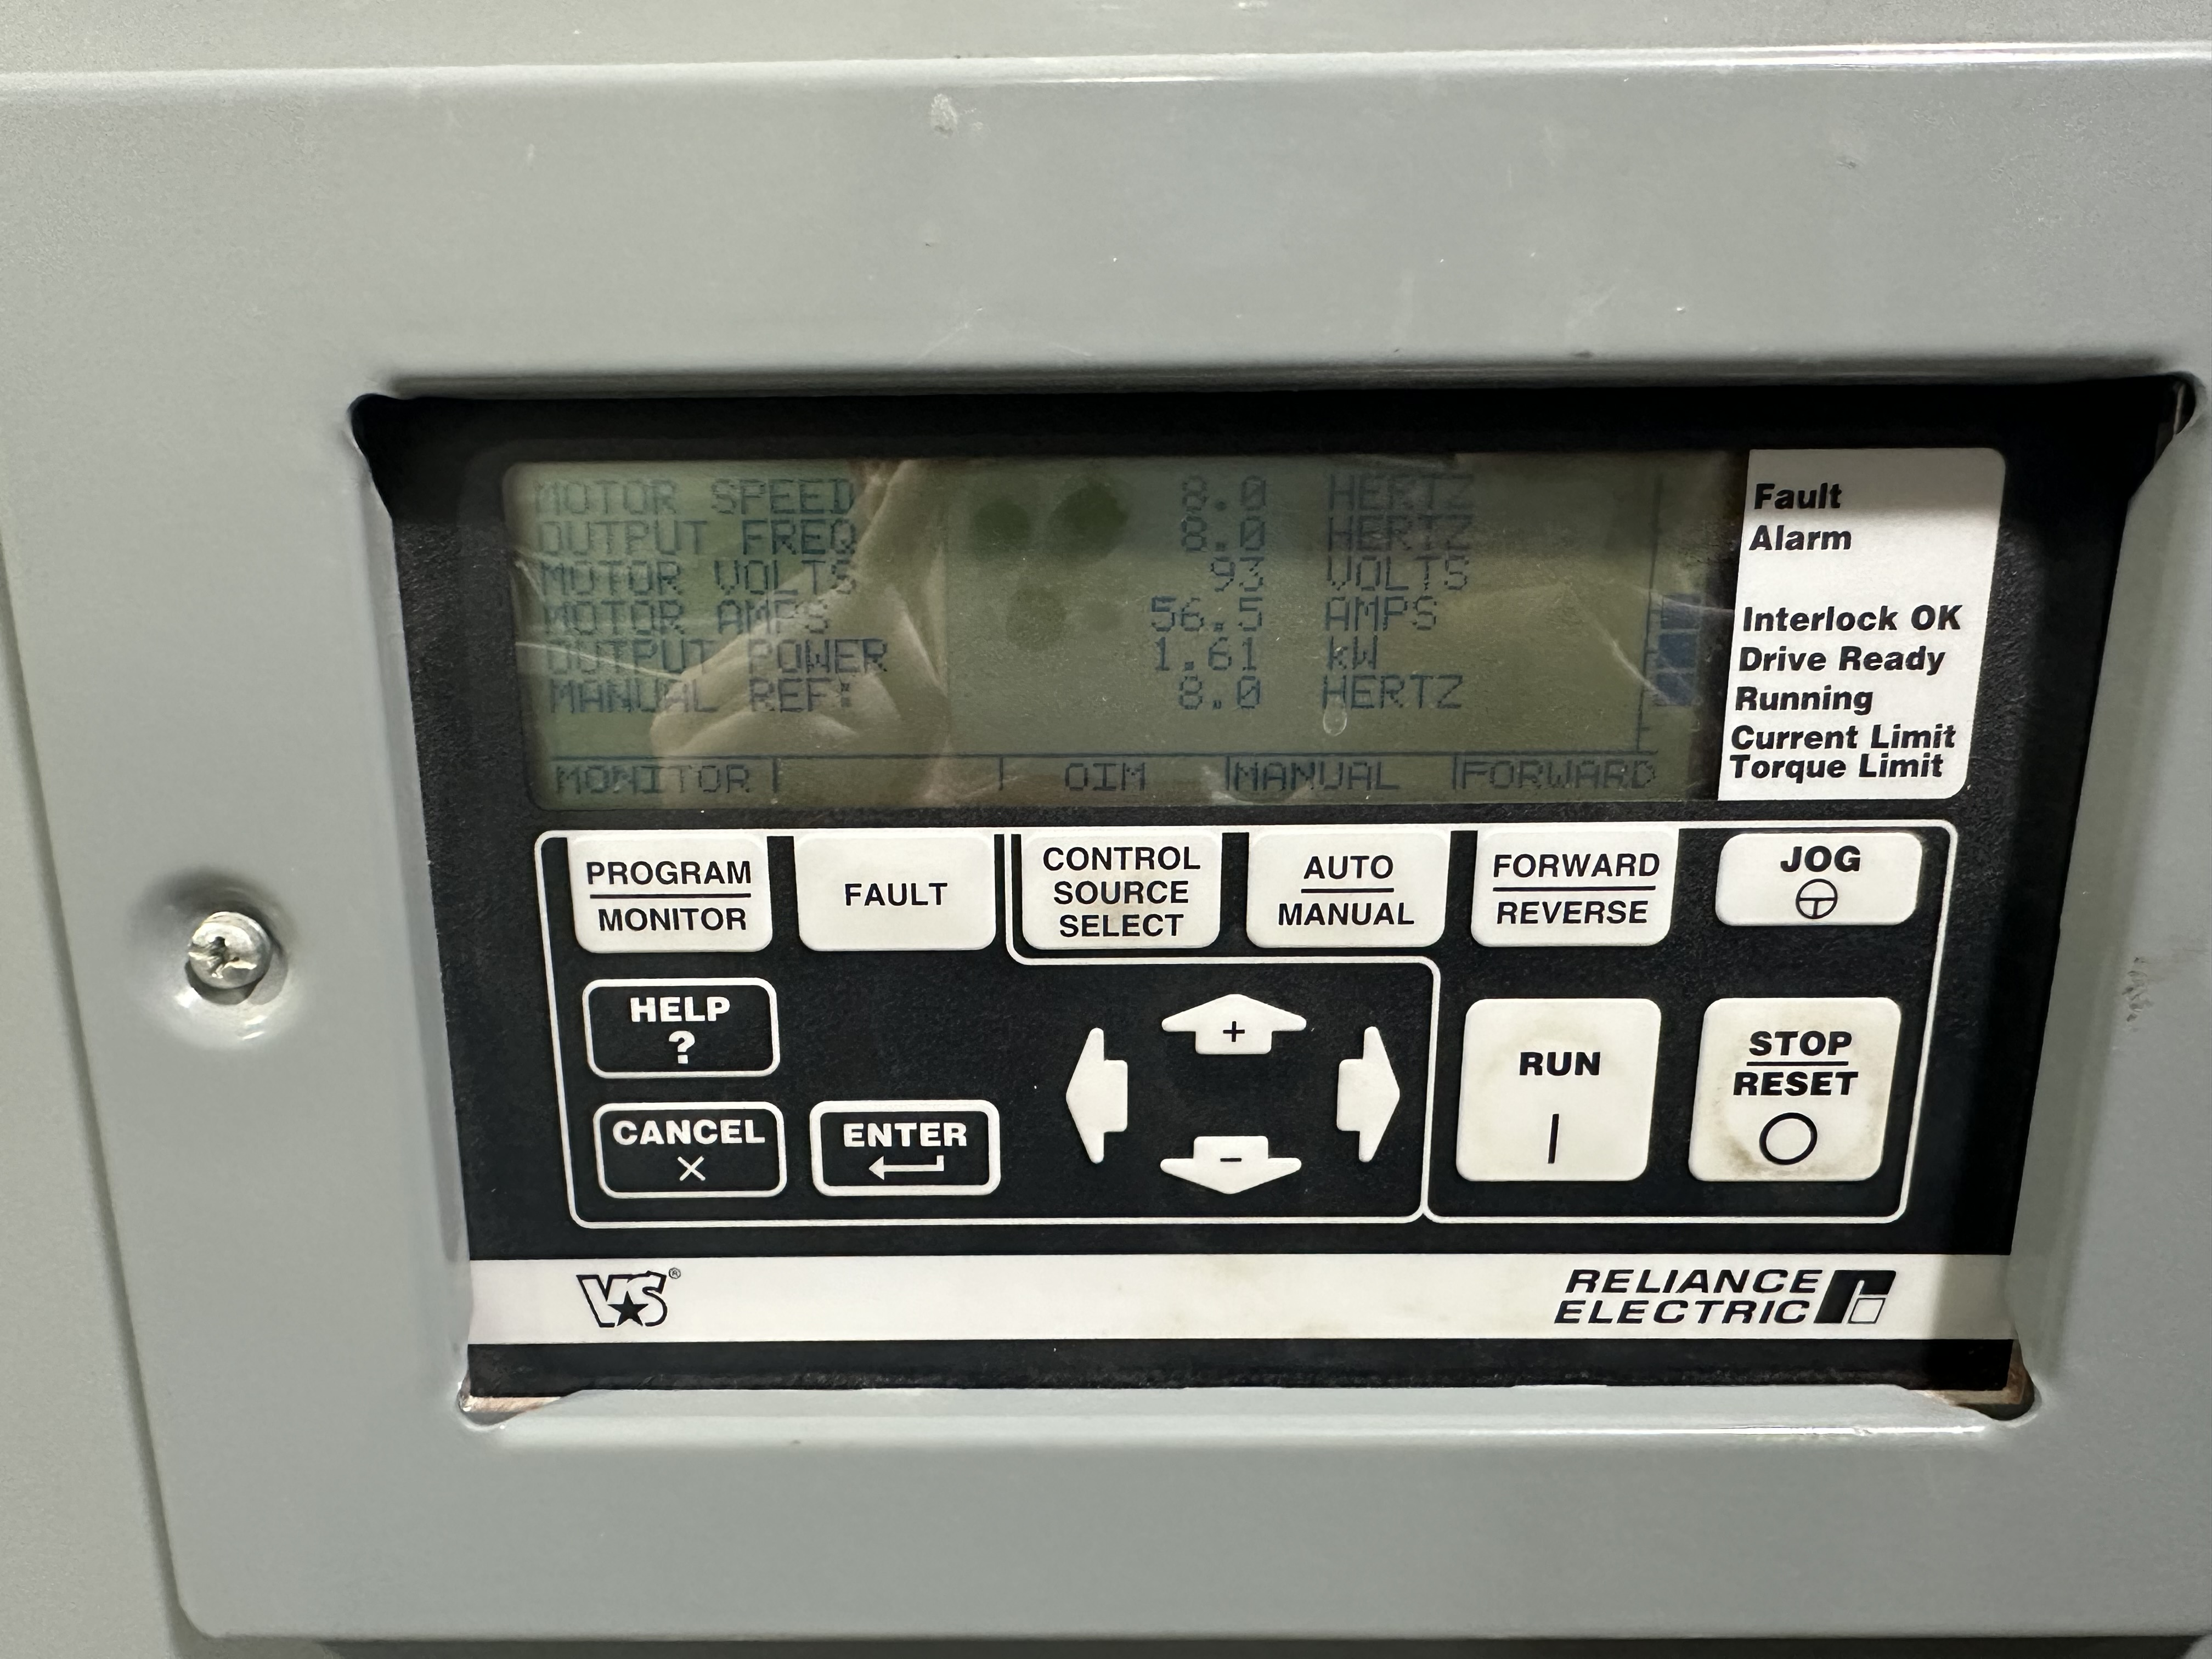
\includegraphics[width=0.75\linewidth]{Figures/IMG_0007.jpeg}
    \caption[Picture of the control panel for wind tunnel]{Picture of the control panel for wind tunnel}
    \label{fig: WindTunnelControl }
\end{figure}

\begin{figure}[htpb]
    \centering
    \includegraphics[width=0.75\linewidth]{Figures/IMG_0008.jpeg}
    \caption[Picture of the Computer program that we used for collecting the data.]{Picture of the Computer program that we used for collecting the data.}
    \label{fig: DataCollectionTool}
\end{figure}

\newpage

\section{Additional Figures} \label{sec:additional_figures}

%\begin{figure}[htpb]
%    \centering
%     \includesvg[width=0.75\linewidth]{Figures/}
%     \caption[A graph of the single-sided amplitude spectrum inside %and outside the wake at a eight degree angle of attack.]{The single-%sided amplitude spectrum inside and outside the wake region at a %\qty{8}{\degree} \acrshort{aoa}.}
%     \label{fig:SSAS_at_8AoA}
%\end{figure}
